%   % !TEX root = ../../VIII,3_Rahmen-TeX_9-0.tex
%  
%   Band VIII, 3 N.~?? 	Stoß
%   Signatur/Tex-Datei:	LH_37_05_153-154
%   RK-Nr. 	57277
%				
%   Überschrift: 	(keine)
%   Titel: 			??			(unser Titel)					??
%   Datierung:		???? bis ???? (a. St.?), eigh. (?)				??
%   Textfolge: 					(ggf. wie Foliierung)				??
%   WZ: 	Falz, Nr. 803046
%   edlabels:			11		(wieviele?)
%   Diagramme: 		4		(wieviele?)					??
%   Dateien (PDF):
%   		LH_37_05_153-154_d1_153r;					
%   		LH_37_05_153-154_d2_153r;					
%   		LH_37_05_153-154_d3_153r;					
%   		LH_37_05_153-154_d4_154r
%
%   Erstaufnahme:			(wer?)
%   Bearbeitung MS ab: 		Juli 2020
%
%   NB: 						(Anmerkungen)					??
%
%
%
\selectlanguage{ngerman}
\frenchspacing
%
\begin{ledgroupsized}[r]{120mm}
\footnotesize
\pstart
\noindent\textbf{Überlieferung:}
\pend
\end{ledgroupsized}
%
\begin{ledgroupsized}[r]{114mm}
\footnotesize
\pstart \parindent -6mm
\makebox[6mm][l]{\textit{L}}%
Konzept:
LH~XXXVII~5~Bl.~153\textendash154. 
Ein Bogen~4\textsuperscript{o};
Wasserzeichen im Falz;
Papiererhaltungsmaßnahmen.
Vier Seiten.
\pend
\end{ledgroupsized}
%
\begin{ledgroupsized}[r]{114mm}
\footnotesize
\pstart
\parindent -6mm
\makebox[6mm][l]{\textit{E}}%
(tlw.) \cite{01056}\textsc{Fichant} 1994, S.~399\textendash402.
\pend%
\end{ledgroupsized}
%
%
\vspace{5mm}
\begin{ledgroup}
\footnotesize
\pstart
\noindent%
\textbf{Datierungsgründe:} %%
Im vorliegenden Konzept bedient sich Leibniz der auf dem Relativitätsprinzip beruhenden Methode zur Stoßanalyse,
%
die er in N.~\ref{RK57269} vom 10.\ (20.) Juni 1677 durch die Schiffsanalogie veranschaulicht hatte.
%
Ein wesentlicher Unterschied zwischen jenem Stück und N.~\ref{RK57277} besteht allerdings in der Haltung,
%
die Leibniz gegenüber dieser Methode an den Tag legt.
%
In N.~\ref{RK57269} diente die Besprechung der Bewegung und des Stoßes zweier Körper auf einem fahrenden Schiff dazu,
%
ein möglichst geeignetes, deutliches Beispiel für die Gefahren des Relativitätsprinzips anzuführen.
%
Daraufhin hatte Leibniz auch seine Vorzüge, und die des Schiffsmodells, für die Stoßanalyse dargetan.
%
In N.~\ref{RK57277} (siehe S.~\refpassage{37_05_153-154_10a}{37_05_153-154_10b}) 
%
tritt an die Stelle des früheren Misstrauens eine durchaus positive Bewertung der Schiffsmethode:
%
Er findet, dass sie einen \glqq überaus schönen wie einfachen\grqq\ Ansatz zur Stoßanalyse an die Hand gibt
(\glqq pulcherrima facillimaque illinc constructio habebitur, ope ejusdem navis, tum facilis habebitur motus resolutio\grqq),
%
dass mit ihrer Hilfe endlich alle Fragen beantwortet sind (\glqq omnia plane absoluta nunc tandem habemus \grqq),
%
und ist sich ihres Hauptergebnisses, dass nämlich abzüglich der Bewegung des gemeinsamen Schwerpunkts
%
die Geschwindigkeiten beider Körper vor und nach dem Stoß im Betrag gleich sind,
%
sicher (\glqq manifeste patet eandem semper esse separationis celeritatem, quae erat concursus\grqq).
%
%
Dieser Umstand deutet auf eine Entwicklung von Leibnizens Position nach der Abfassung von N.~\ref{RK57269} und spricht für
%
die Enstehung von N.~\ref{RK57277} ab Ende Juni 1677.
%
Die Formeln, die Leibniz am Ende seiner Schiffsanalyse am freigebliebenen rechten Rand von Bl.~154~v\textsuperscript{o} 
geschrieben hat (S.~\refpassage{37_05_153-154_7a}{37_05_153-154_7b}) entsprechen, wie von \textsc{Fichant} 1994 (S.~401f.) festgestellt, den klassischen Gleichungen der Geschwindigkeiten beim vollkommen elastischen Stoß zweier Körper.
%
\pend
%
\pstart
Die Tatsache, dass Leibniz die \textit{vis} mit der Bewegungsgröße gleichsetzt 
(siehe S.~\refpassage{37_05_153-154_11a}{37_05_153-154_11b}),
ist ein Indiz der Entstehung von N.~\ref{RK57277} vor \textit{De corporum concursu}, \textit{Scheda octava} von Januar 1678 (N.~\ref{dcc_08}).
Daraus ergibt sich die vorgeschlagene Datierungsspanne: Ende Juni 1677 bis Januar 1678.
\pend
%
\pstart
Innerhalb dieser Zeitspanne lässt sich abschließend die relative Datierung von N.~\ref{RK57277} gegenüber N.~\ref{RK57275} feststellen.
%
Im vorliegenden Konzept geht Leibniz von der These der gleichförmigen Bewegung des \textit{centrum potentiae} aus,
%
die er sogar an verschiedenen Stellen zu beweisen versucht.
%
Dass diese Gesetzmäßigkeit in ihrer allgemeinen Form nicht haltbar ist, wie er in N.~\ref{RK57275} an einem Beispiel zeigt,
%
scheint ihm in N.~\ref{RK57277} nicht bekannt zu sein, was auf die frühere Entstehung
%
des vorliegenden Konzepts gegenüber N.~\ref{RK57275} schließen lässt.
%
\pend 
\end{ledgroup}
%
\newpage%
%
\selectlanguage{latin}
\frenchspacing
\vspace{8mm}
\pstart%
\normalsize%
\noindent%
\lbrack153~r\textsuperscript{o}\rbrack\
\pend
%
%
\vspace{1.0em} %%%%%%%%% Diagramm 1
\centerline{%
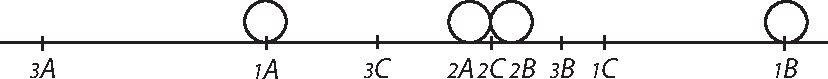
\includegraphics[width=0.85\textwidth]{%
gesamttex/edit_VIII,3/images/LH_37_05_153-154_d1_153r.pdf%
}} 
\vspace{0.5em}
\centerline{%
\lbrack\textit{Fig.~1}\rbrack%
}
% \newpage%
\vspace{1.5em}
%
%%%%%%%%% Diagramm 2
\centerline{%
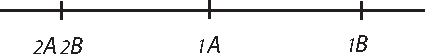
\includegraphics[width=0.5\textwidth]{%
gesamttex/edit_VIII,3/images/LH_37_05_153-154_d2_153r.pdf%
}} 
\vspace{0.2em}
\centerline{%
\lbrack\textit{Fig.~2}\rbrack%
}
% \newpage%
\vspace{1em}
%
%%%%%%%%% Diagramm 3
\centerline{%
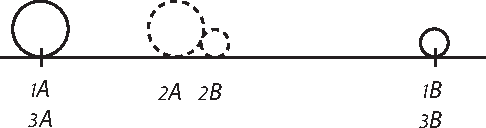
\includegraphics[width=0.58\textwidth]{%
gesamttex/edit_VIII,3/images/LH_37_05_153-154_d3_153r.pdf%
}} 
\vspace{0em}
\centerline{%
\lbrack\textit{Fig.~3}\rbrack%
}
% \newpage%
\vspace{1em}
%
\pstart
\noindent ${\scriptstyle \textit{1}}B{\scriptstyle \textit{1}}C \, \sqcap \, al$. 
%%%%%%% ---------------
\edtext{${\scriptstyle \textit{1}}A{\scriptstyle \textit{1}}C \, \sqcap \, bl.$ ${\scriptstyle \textit{1}}A{\scriptstyle \textit{2}}A\, \sqcap\,e$.}{\lemma{${\scriptstyle \textit{1}}A{\scriptstyle \textit{1}}C \, \sqcap \, bl.$}\Bfootnote{\textbar\ ${\scriptstyle \textit{1}}B{\scriptstyle \textit{2}}B \,\sqcap\,f$ \textit{gestr.}\ \textbar\ \textit{{\scriptsize1}A{\scriptsize2}A}~\textit{L}}} 
%%%%%%% ---------------
${\scriptstyle \textit{1}}B{\scriptstyle \textit{2}}B\,\sqcap\,f. \ {\scriptstyle \textit{3}}A {\scriptstyle \textit{2}}A\,\sqcap\,i. \ {\scriptstyle \textit{3}}B {\scriptstyle \textit{2}}B\,\sqcap\,m.$
\pend
%
\pstart\noindent
%
\rule[0cm]{0mm}{12pt}${\scriptstyle \textit{1}}C{\scriptstyle \textit{2}}C\,\sqcap\, {\scriptstyle \textit{2}}C {\scriptstyle \textit{3}}C\,\sqcap\,c. \ {\scriptstyle \textit{2}}B{\scriptstyle \textit{2}}A\,\sqcap\,h.$
\pend \pstart
%
\hspace{1mm}\hspace{-1mm}% Trick, weil \edlabel nicht zu \par-Beginn sein darf
\edlabel{37_05_153-154_1a}%	A-Fn. Randanmerkung
\edtext{}{%
{\xxref%
{37_05_153-154_1a}{37_05_153-154_1b}}%
\lemma{}%
\Afootnote{%
\textit{Am Rand:} $ai+bf\,\sqcap\,ai+bf$, si $e\,\sqcap\,i$ et $f\,\sqcap\,m$. Ergo $ai-ai\,\sqcap\,bf-bf$. 
Ergo 
$\displaystyle\frac{a}{b}\,\sqcap\,\displaystyle\frac{i-i}{f-f}$, 
\protect\rule[0cm]{0mm}{16pt}seu 
$\displaystyle\frac{i-i}{f-f}-\frac{a}{b}\,\sqcap\,0$ seu $i-i-\displaystyle\frac{a}{b}\,\smallfrown\,f-f\,\sqcap\,0$. 
\newline
Est autem $f-f\,\sqcap\,i-i$. 
\protect\rule[0cm]{0mm}{16pt}Fit ergo $i-i,-,\overline{i-i}\displaystyle\frac{a}{b}$. 
Seu fit $i-i,\smallfrown\,1-\displaystyle\frac{a}{b}\,\sqcap\,0$. 
Ergo si 
$m-f\,\sqcap\,e-i\,\sqcap\,0$, 
tunc consequitur esse 
$1-\displaystyle\frac{a}{b}\,\sqcap\,0$. 
Si $0\,\sqcap\,0$ 
fiet $\displaystyle\frac{a}{b}\,\sqcap\,\displaystyle\frac{f-m}{i}$,
et $i\,\sqcap\,f+m$.
Ergo $\displaystyle\frac{a}{b}\,\sqcap\,\displaystyle\frac{f-m}{f+m}$. $fa+ma\,\sqcap\,fb-mb$. 
Ergo 
$m\,\sqcap\,\displaystyle\frac{fb-fa}{a+b}$, 
$f-m\,\sqcap\,\displaystyle\frac{2f\lbrack a\rbrack}{a+b}.\efrac{\textsuperscript{\lbrack a\rbrack}}{}$
\newline\newline%Marginalienapparat:
{\footnotesize \textsuperscript{\lbrack a\rbrack} $\displaystyle\frac{2fb}{a+b}$. \textit{L\ ändert Hrsg.}}%
}}%
%	Ende A-Fn. Randanmerkung
\edtext{Ex natura potentiae absolutae,\protect\index{Sachverzeichnis}{potentia absoluta}}{%
\lemma{}%
\Bfootnote{%
Ex natura potentiae absolutae, %
\textit{erg.~L}}}
$\overset{\displaystyle (1)}{ae+bf\,\sqcap\,ai+bm}$. 
Ergo 
$ae-ai\,\overset{\displaystyle (2)}{\sqcap}\,bm-bf$. 
Ergo 
$\displaystyle \frac{a}{b}\, \overset{\displaystyle (3)}{\sqcap}\,\displaystyle \frac{m-f}{e-i}$. 
$\overset{\displaystyle (4)}{{\scriptstyle \textit{1}}B{\scriptstyle \textit{1}}A\,\sqcap\,{\scriptstyle \textit{3}}B {\scriptstyle \textit{3}}A}$ 
%% ----------------
\edtext{ex natura mutationis respectivae.\protect\index{Sachverzeichnis}{mutatio respectiva}}{\lemma{}\Bfootnote{ex natura mutationis respectivae \textit{erg.~L}}} 
%% ---------------
${\scriptstyle \textit{1}}B{\scriptstyle \textit{1}}A\,\overset{\displaystyle (5)}{\sqcap}\,\underset{\displaystyle f}{{\scriptstyle \textit{1}}B{\scriptstyle \textit{2}}B}+\underset{\displaystyle h}{{\scriptstyle \textit{2}}B{\scriptstyle \textit{2}}A}\,\leibdashv\,\underset{\displaystyle e}{{\scriptstyle \textit{2}}A{\scriptstyle \textit{1}}A}$, 
posito \textit{B} esse corpus quod 
%% ---------------
\edtext{non praecedit}{\lemma{non}\Bfootnote{\textit{(1)}~sequitur \textit{(2)}~praecedit~\textit{L}}}
%
\textit{A}, 
%
sed vel ei sequitur, \edtext{quo casu est $\pleibdashv\,\sqcap\,-$ \lbrack,\rbrack}{\lemma{}\Bfootnote{quo casu est $\pleibdashv\,\sqcap\,-$ \textit{erg.~L}}} 
%% ---------------
vel ipsi occurrit\lbrack,\rbrack\
%% ---------------
\edtext{quo casu est $\pleibdashv\,\sqcap\,+$}{\lemma{}\Bfootnote{quo casu est $\pleibdashv\,\sqcap\,+$ \textit{erg.~L}}}. 
%% --------------
Ergo ${\scriptstyle \textit{1}}B{\scriptstyle \textit{1}}A\,\sqcap\,f+h\,\pleibdashv\, e$. 
Tantum suppono \textit{{\scriptsize1}A} non cadere inter \textit{{\scriptsize2}A} et \textit{{\scriptsize2}B}, 
quod obtinetur, si diuturnus satis assumatur motus.\protect\index{Sachverzeichnis}{motus satis diuturnus} 
Cumque semper fingi possit 
\rule[0cm]{0mm}{12pt}diutius durasse, eodem manente effectu, ideo casus iste praeteriri potest.
\pend
%
\pstart
%% ========= 
\rule[0cm]{0mm}{16pt}${\scriptstyle \textit{3}}B {\scriptstyle \textit{3}}A\,\sqcap\,\parbox[t][1.2cm][c]{3.55cm}{\vspace{-4mm} 
$\begin{array}{c} \underset{\displaystyle \textup{cum}\ B \ \textup{regreditur}\protect\rule[0cm]{0mm}{10pt}}{+{\scriptstyle \textit{3}}B{\scriptstyle \textit{2}}B+{\scriptstyle \textit{2}}B{\scriptstyle \textit{2}}A +{\scriptstyle \textit{2}}A {\scriptstyle \textit{3}}A},\\ \underset{\displaystyle\textup{cum}\ B \ \textup{procedit}\protect\rule[0cm]{0mm}{10pt}}{-{\scriptstyle \textit{3}}B{\scriptstyle \textit{2}}B+{\scriptstyle \textit{2}}B{\scriptstyle \textit{2}}A +{\scriptstyle \textit{2}}A {\scriptstyle \textit{3}}A} \end{array}$}$\quad 
%% ==========
seu 
${\scriptstyle \textit{3}}B{\scriptstyle \textit{3}}A\,\overset{\displaystyle (6)}{\sqcap}\,(\pleibdashv)\,m+h+i$.
%
%
\pend
%
\pstart
Ergo per 4.~5.~6.\ aeqq.\ erit 
$f\,\ovalbox{$+h$}\,\pleibdashv e\,\overset{\displaystyle (7)}{\sqcap}\,(\pleibdashv)m\,\ovalbox{$+h$}+i$ 
seu erit 
$f\,\pleibdashv\,e\,\overset{\displaystyle (8)}{\sqcap}\,(\pleibdashv)\,m+i$. 
%
Seu 
$i\,\pleibvdash \,e\,\overset{\displaystyle (9)}{\sqcap}\,f\,(\pleibvdash) \,m$ 
seu 
$\displaystyle \frac{i\,\leibvdash \,e}{f\,(\leibvdash)\,m}\,\overset{\displaystyle (10)}{\sqcap}\,1$, 
quam aequationem conferendo cum aequatione 3.\ et 
\rule[0cm]{0mm}{10pt}supponendo \textit{a} et \textit{b} corpora esse inaequalia, 
non potest esse $\pleibvdash\,\sqcap\,-$ ita ut simul sit etiam $(\pleibvdash)\,\sqcap\,-$.%
\edlabel{37_05_153-154_1b}	%Ende A-Fn. Randanmerkung
%
Foret enim 
$\displaystyle\frac{i-e}{f-m}\,\sqcap\,1$, 
sed idem 
$\sqcap\,\displaystyle \frac{a}{b}$, 
ergo 
\edtext{$\displaystyle\frac{a}{b}\,\sqcap\,1$, seu $a\,\sqcap\,b$, quod est}{\lemma{}\Afootnote{\textit{Oberhalb der Zeile, im Anschluss an} seu $a\,\sqcap\,b$:\enspace vel saltem $m-f\,\sqcap\,0$ et $e-i\,\sqcap\,0$}}
%
contra
%
%	
\edlabel{37_05_153-154_3a}%
\edtext{}{% Große Streichung
{\xxref%
{37_05_153-154_3a}{37_05_153-154_3b}}%
\lemma{hypothesin.}%
\Bfootnote{%
\textbar\ Jam \lbrack...\rbrack\ $i-e\,\sqcap\,f+m$. \textit{erg.}~\textbar\
Eademque vice $i+e\,\sqcap\,m-f$. Ergo $i\,\sqcap\,f$ et $e\,\sqcap\,m$.  
Ergo $i\,\sqcap\,m$. $a\,\sqcap\,b$. \textit{erg.\ u.\ gestr.}~\textbar\ %
\textit{(1)}~Superest ut examinemus an unum signum possit esse $+$, alterum minus. 
Sit ergo $\pleibvdash\,\sqcap\,+$ et $(\pleibvdash)$ sit $-$.
Fiet $\displaystyle\frac{i+e}{f-m}\,\sqcap\,1$ seu $f-m\,\sqcap\,i+e$ 
seu $f-e\,\sqcap\,i+m$. 
Sed etiam ex aequ.\ 3.\ 
$f-m\,\sqcap\,\overline{i-e}\,\displaystyle\frac{a}{b}$. 
Ergo $\overline{i-e}\displaystyle\frac{a}{b}\,\sqcap\,i+e$. 
Ergo $ai-ae\,\sqcap\,bi+be$. 
Ergo $ai-bi\,\sqcap\,ae+be$. 
Est autem $ai\,\sqcap\,ae+bf-bm$. 
\textbar\ per aequ.\ 1.\ \textit{erg.}\ \textbar\
Ergo fiet:  
$\protect\ovalbox{\textit{ae}}+bf-bm-bi\,\sqcap\, \protect\ovalbox{\textit{ae}}+be$. 
Ergo fiet: 
$f-m-i\,\sqcap\,e$, seu $i+m\,\sqcap\,e-f$ 
quod est absurdum si ponamus celeritatem ipsius \textit{B}, \textit{f}, esse majorem, quam ipsius \textit{A} celeritatem, \textit{e}. 
Similiter ponamus 
\mbox{$\pleibvdash$ esse $-$} et 
\mbox{$(\pleibvdash)$ esse $+$.} 
Fiet $\displaystyle\frac{i-e}{f+m}\,\sqcap\,1$ 
seu $i-e\,\sqcap\,f+m$. 
Sed etiam ex aequ.\ 3.\ $f-m\,\sqcap\,\overline{i-e}\,\displaystyle\frac{a}{b}$. 
Ergo $\overline{i-e}\displaystyle\frac{a}{b}\,\sqcap\,i+e$. 
Ergo $ai-ae\,\sqcap\,bi+be$. 
Jam ex aequ. 1\textsuperscript{ma} est $ai\,\sqcap\,ae+bf-bm$ quo valore in aequatione praecedente substituto, 
fiet 
%% ----------
$\protect\underset{\protect\overbrace{\displaystyle{\protect\raisebox{-1.95mm}{\protect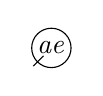
\begin{tikzpicture} \protect\draw (0,0) circle (0.25cm) node at (0,0) {\textit{ae}}; \protect\draw (-.23,-.23) -- (-.1,-.1); \protect\end{tikzpicture}}+bf-bm}}}{ai} \protect\raisebox{-2.2mm}{\protect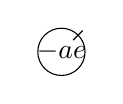
\begin{tikzpicture} \protect\draw (0,0) circle (0.3cm) node at (0,0) {$-ae$}; \protect\draw (.15,.15) -- (.27,.27); \protect\end{tikzpicture}}\,\sqcap\,bi+be$, 
%% ----------
seu dividendo per \textit{b} erit 
$f-m\,\sqcap\,i+e$. 
Sed hoc fieri non potest si \textit{m} sit major quam \textit{f}, intelligi autem semper potest \textit{m} major quam \textit{f}, quando corpora concurrunt,
\textit{(a)}~ergo
\textit{(b)}~tunc enim nihil refert ad hunc calculum, quodnam ex his corporibus vocetur \textit{B} aut \textit{A}. 
Appellando ergo \textit{A} illud cujus celeritas \textit{e}, major est, utique absurda erit aequatio $f-e\,\sqcap\,i+m$. 
Est autem eo casu ut
\textit{(aa)}~aliunde
\textit{(bb)}~notum ex superioribus $\pleibvdash\,\sqcap\,+$. Ergo ponendo $(\pleibvdash)\,\sqcap$ 
\textit{(2)}~Ergo si corpora concurrunt, necessario aut corpora aequalia  %
\textit{(3)}~Ergo \lbrack...\rbrack\ signo $-$. %
\textit{L}%
}}%
hypothesin. Jam si corpora concurrant $\pleibvdash$ est $\sqcap\,-$.
Ergo si corpora concurrant $(\pleibvdash)$ necessario est $+$, et fiet 
$i-e\,\sqcap\,f+m$.
\pend
%
\pstart
Ergo si corpora sibi concurrant, tunc vel aequalia sunt corpora, vel aequales sunt vires,\protect\index{Sachverzeichnis}{vis} vel aliquod ex ipsis progreditur, cujus celeritas
%
\edtext{quaesita}{\lemma{}\Bfootnote{quaesita \textit{erg.~L}}}
affecta erit signo\protect\index{Sachverzeichnis}{signum} $-$.%
\edlabel{37_05_153-154_3b}
\pend \pstart
%
%
%%%%%%%%%%%%%%%%%%%%%%%%%%%%%%%%%
%
% E N D  O F  1 5 3 R =====
%
%%%%%%%%%%%%%%%%%%%%%%%%%%%%%%%%%
%
%
%
%%%%%%%%% ==== F O L . 1 5 3  V E R S O ==== %%%%%%%%%%%
%
%
%
%
\lbrack153~v\textsuperscript{o}\rbrack\
Si vero unum corpus praecedat alterum sequatur, tunc $\pleibvdash$ necessario est $+$, 
et tunc si poneremus $(\pleibvdash)$ esse $+$ fieret $\displaystyle\frac{i+e}{f+m}\,\sqcap\,1$ seu 
%
%
\edtext{%
$i+e\,\sqcap\,f+m$. Cum autem $(\pleibvdash)$ est $+$, seu cum $(\pleibdashv)$ est $-$\lbrack,\rbrack\ tunc corpus impingens\protect\index{Sachverzeichnis}{corpus impingens} 
progreditur. Si vero ($\pleibvdash$) sit $-$\lbrack,\rbrack\ tunc corpus impingens\protect\index{Sachverzeichnis}{corpus impingens} reflectitur.}%
{\lemma{$i+e\,\sqcap\,f+m$.}\Bfootnote{%
\textit{(1)}~Quod scilicet continget, si
\textit{(a)}~corpus antecedens
\textit{(b)}~corpus impingens reflectatur, nam antecedens semper pergit  cum nihil repellat. Si vero cor
\textit{(2)}~Est 
\textit{(3)}~Cum autem \lbrack...\rbrack\ reflectitur.~\textit{L}}} 
%
Cum enim antecedens\protect\index{Sachverzeichnis}{corpus antecedens} semper pergat, hinc redeunte impingente, corpora a se invicem divergunt, ac signorum\protect\index{Sachverzeichnis}{signum} idem est status, 
%
\edtext{ac si concurrerent. Tantum examinandum}{\lemma{ac si}\Bfootnote{\textit{(1)}~divergerent \textit{(2)}~concurrerent. \textit{(a)}~Si vero impingens \textit{(aa)}~occurrat, tunc \textit{(bb)}~pergat, tunc \textit{(b)}~Tantum~\textit{L}}} 
%
est, 
%
\edtext{quando impingens\protect\index{Sachverzeichnis}{corpus impingens} reflectatur vel}{\lemma{quando}\Bfootnote{\textit{(1)}~corpora \textit{(2)}~impingens reflectatur \textit{(a)}~vel non, quod videtur non ex \textit{(b)}~vel~\textit{L}}}
%
non. 
%
Et quidem si sit $\displaystyle\frac{i+e}{f-m}\,\sqcap\,1$ seu 
%
\edtext{$f-m\,\sqcap\,i+e$ vel}{\lemma{$f-m\,\sqcap\,i+e$}\Bfootnote{\textit{(1)}~. Erit necessario \textit{(2)}~vel~\textit{L}}} 
%
$f-e\,\sqcap\,i+m$ debet necessario esse \textit{f} major 
%
%
\edlabel{37_05_153-154_8a}%
\edtext{}{%
{\xxref%
{37_05_153-154_8a}{37_05_153-154_8b}}%
\lemma{quam \textit{e}.}%
\Bfootnote{%
\textit{(1)}~Itaque si ce \textit{(2)}~Id~\textit{L}}}%
quam \textit{e}. 
%
\edtext{Id\edlabel{37_05_153-154_8b}
vero verum esse aliunde patet\lbrack,\rbrack}{%
\lemma{Id \lbrack...\rbrack\ aliunde patet}%
\Cfootnote{%
Das beschriebene Verhältnis zwischen den Geschwindigkeiten \textit{e} und \textit{f} ist eigentlich tautologisch.%
}}
%
alioqui enim corpus \textit{B} non assequeretur corpus \textit{A}, nisi celerius 
%
\edtext{moveretur. Porro}{\lemma{moveretur}\Bfootnote{\textit{(1)}~, ergo si corpus \textit{B} sequatur corpus \textit{A}, necessario etiam erit corporis \textit{B} celeritas per ictum \textit{(2)}~. Porro~\textit{L}}} 
%
si corpus \textit{B} reflectitur, tunc necessario debet celeritas \textit{B} per ictum diminui. %
\pend
%
\pstart
Imo manifeste patet $f\,\groesser\,m$ et $i\,\groesser\,a$ quandocunque \textit{B} sequitur \textit{A}, utique enim augebit necessario celeritatem ipsius \textit{A}, in eam partem, in quam impellitur, aucta autem celeritate ipsius \textit{A}, celeritatem ipsius \textit{B} minui manifestum est. 
%
%
\pend
%
\pstart
Ante omnia porro manifestum est, si persequens\protect\index{Sachverzeichnis}{corpus persequens} sit majus antecedente,\protect\index{Sachverzeichnis}{corpus antecedens} non repelli
%
\edtext{sed progredi}{\lemma{}\Bfootnote{sed progredi \textit{erg.~L}}},
%
si sit aequale, videtur in ejus locum, quod propellit, quiescere, nam, sive quiescat, sive progrediatur, id quod impellitur, idem 
%
\edtext{est, non}{\lemma{est,}\Bfootnote{\textit{(1)}~perinde \textit{(2)}~ob mo \textit{(3)}~non~\textit{L}}} 
%
magis enim ab eo patitur, quam in ipsum agit, ergo concludo, si corpus minus majori antecedenti impingat, semper repelli. 
%
% ====
\pend \pstart
% ====
%
Possunt autem ista omnia praeclare demonstrari per motuum compositiones.\protect\index{Sachverzeichnis}{compositio motuum}
Exempli causa 
%
\edtext{pono corpus}{\lemma{}\Bfootnote{pono \textit{(1)}~utrumque \textit{(2)}~corpus~\textit{L}}} 
%
quiescens in navi\protect\index{Sachverzeichnis}{navis} esse, et aliud in ipsum impingere, navem\protect\index{Sachverzeichnis}{navis} 
%
autem progredi, patet spectantibus in ripa\protect\index{Sachverzeichnis}{spectantes in ripa} 
%
motum appariturum, quem dixi, corporis corpus persequentis,\protect\index{Sachverzeichnis}{corpus persequens} 
%
et phaenomena quae dixi necessario eventura. Ex uno hoc 
%
\edtext{principio compositionis}{\lemma{principio}\Bfootnote{\textit{(1)}~compositionibus \textit{(2)}~compositionis~\textit{L}}}
%
motuum, etiam poterunt demonstrari caetera, modo caveamus ne augeamus minuamusve potentiam. 
Nimirum cum certum sit corpora 
%
\edtext{reciprocis ponderi}{\lemma{reciprocis}\Bfootnote{\textit{(1)}~moli \textit{(2)}~ponderi~\textit{L}}} 
%
celeritatibus\protect\index{Sachverzeichnis}{celeritates reciprocae ponderi} concurrentia aequali celeritate repelli, ponamus id fieri in nave\protect\index{Sachverzeichnis}{navis} mota, et spectari e ripa.\protect\index{Sachverzeichnis}{ripa} 
Inde facile habebimus omnia phaenomena concursuum\protect\index{Sachverzeichnis}{phaenomena concursuum} 
%
nec ullo modo augebitur potentia.\protect\index{Sachverzeichnis}{potentia}
% 
Hinc statim etiam demonstratur in eadem necessario recta progredi centrum gravitatis,\protect\index{Sachverzeichnis}{centrum gravitatis} quia 
%
\edtext{fingendo corpora reciproca moli celeritate\protect\index{Sachverzeichnis}{celeritates reciprocae moli} procedere, 
utique centrum gravitatis\protect\index{Sachverzeichnis}{centrum gravitatis} eorum in eadem semper recta
progreditur uniformiter,\protect\index{Sachverzeichnis}{progressus uniformis centri gravitatis in recta}}{\lemma{fingendo \lbrack...\rbrack\ uniformiter}\Cfootnote{Wenn die Geschwindigkeiten reziprok zu den Massen sind, ruht der Schwerpunkt.}} 
%
idem autem progreditur et cum navi\protect\index{Sachverzeichnis}{navis} uniformiter.
%
Ergo motus\protect\index{Sachverzeichnis}{motus uniformis} ex duobus uniformibus compositus\protect\index{Sachverzeichnis}{motus ex duobus uniformibus compositus} motibus est etiam uniformis. 
%
\edlabel{37_05_153-154_6a}%			% Zwecks Referenzierung
Hinc porro demonstratur, et centrum potentiae\protect\index{Sachverzeichnis}{centrum potentiae} in eadem progredi recta uniformiter,\protect\index{Sachverzeichnis}{progressus uniformis centri potentiae in recta} 
%
\edtext{quia si corpora %C-Fn umschließt B-Fn
%
\edtext{fingantur concurrere}{\lemma{fingantur}\Bfootnote{\textit{(1)}~aequaliter concurrere hoc centrum potentiae \textit{(2)}~concurrere~\textit{L}}} 
%
celeritatibus reciproce proportionalibus\protect\index{Sachverzeichnis}{celeritates reciproce proportionales} quiescet hoc centrum,\protect\index{Sachverzeichnis}{centrum potentiae}}{\lemma{quia \lbrack...\rbrack\ centrum}\Cfootnote{Eigentlich ruht das \textit{centrum potentiae} genau dann, wenn die Geschwindigkeiten der Körper reziprok zu den Bewegungsgrößen (\textit{potentiae}) sind, nicht zu den Massen. Unter den gegebenen Voraussetzungen müssten also die Körper zusätzlich gleiche Massen haben.}}
%
interea navis\protect\index{Sachverzeichnis}{navis} eadem celeritate progredietur.%
\edlabel{37_05_153-154_6b}
%
\pend \pstart
%
%
\lbrack154~r\textsuperscript{o}\rbrack\
%
\edlabel{37_05_153-154_10a}%
Hinc verissima etiam apparet 
\edtext{ratio, quid}{\lemma{ratio,}\Bfootnote{\textit{(1)}~tum cur eadem semper servetur \textit{(2)}~quid~\textit{L}}} 
praestet ictus\protect\index{Sachverzeichnis}{ictus} aut non 
%
\edtext{praestet, et}{\lemma{praestet,}\Bfootnote{\textit{(1)}~nam \textit{(2)}~et~\textit{L}}}
% 
quid fiat, si corpora concurrentia sunt mollia,\protect\index{Sachverzeichnis}{corpora mollia} in quibus ictus\protect\index{Sachverzeichnis}{ictus} perit. 
Item manifeste
%
patet eandem semper esse separationis celeritatem,\protect\index{Sachverzeichnis}{celeritas separationis} quae erat concursus.\protect\index{Sachverzeichnis}{celeritas concursus}
%
Denique omnia plane absoluta nunc tandem habemus, sed necessario ab 
%%
\edtext{Hugenii et Mariotti, et Wallisii et Wrenni}{\lemma{Hugenii \lbrack...\rbrack\ Wrenni}\Cfootnote{%
\protect\index{Namensregister}{\textso{Huygens} (Hugenius, Ugenius, Hugens, Huguens), Christiaan 1629\textendash1695}\textsc{C.~Huygens}, \cite{00529}\glqq Regles du mouvement dans la rencontre des corps\grqq, \cite{00157}\textit{JS} (Pariser Ausgabe), 18.~März 1669, S.~22\textendash24 (\cite{00113}\textit{HO} XVI, S.~179\textendash181); %
\protect\index{Namensregister}{\textso{Mariotte}, Edme, Seigneur de Chazeuil ca. 1620\textendash1684}
\textsc{E.~Mariotte}, \cite{00311}\textit{Traité de la percussion}, Paris 1673; %
\protect\index{Namensregister}{\textso{Wallis} (Wallisius), John 1616\textendash1703}\textsc{J.~Wallis}, \cite{01065}\glqq A summary account \lbrack...\rbrack\ of the general laws of motion\grqq, \cite{00158}\textit{PT} III (1668\textendash1669), Januar 1669, S.~864\textendash866; %
\protect\index{Namensregister}{\textso{Wallis} (Wallisius), John 1616\textendash1703}\textsc{Ders.}, \cite{00301}\textit{Mechanica}, London 1670\textendash1671, Pars~III, Cap.~XI, S.~660\textendash682 (\cite{01008}\textit{WO} I, S.~1002\textendash1015) sowie Cap.~XIII, S.~686\textendash707 (\cite{01008}\textit{WO} I, S.~1018\textendash1031); %
\protect\index{Namensregister}{\textso{Wren} (Wrennus), Christopher 1632\textendash1723}\textsc{C.~Wren}, \cite{01066}\glqq Theory concerning the same subject\grqq, \cite{00158}\textit{PT} III (1668\textendash1669), Januar 1669, S.~867f.%
}}
%%%
regulis diversa.
%
Tandem pulcherrima facillimaque illinc constructio\protect\index{Sachverzeichnis}{constructio pulcherrima facillimaque} habebitur, ope ejusdem navis,\protect\index{Sachverzeichnis}{navis}
%
tum facilis habebitur motus resolutio,\protect\index{Sachverzeichnis}{resolutio facilis motus} atque ita omnia non calculo, sed ratiocinatione transigentur. 
Denique examinari poterit quid fiat, si duae sint naves,\protect\index{Sachverzeichnis}{navis} et 
%
\edtext{duo illis corpora, mota}{\lemma{duo}\Bfootnote{\textit{(1)}~in ips \textit{(2)}~illis corpora,
\textit{(a)}~separatim \textit{(b)}~mota~\textit{L}}} 
%
diverso a navibus motu, et separatim corpora, separatim naves\protect\index{Sachverzeichnis}{navis} sibi infligant 
%
\edtext{ictum. Atque}{\lemma{ictum.}\Bfootnote{\textit{(1)}~Denique \textit{(2)}~Atque~\textit{L}}} 
%
ita denique obtinuimus rem diu quaesitam, ut omnia per solas motuum compositiones,\protect\index{Sachverzeichnis}{compositio motuum} 
%
hoc uno observato, ut ne quid potentiae\protect\index{Sachverzeichnis}{potentia} pereat, explicarentur: videamus tantum qua ratione id semper obtineatur, ne scilicet variari possit 
%
\edtext{motuum}{\lemma{}\Bfootnote{motuum \textit{erg.}~\textit{L}}} 
%
compositionis\protect\index{Sachverzeichnis}{compositio motuum} et phenomenorum modus.%
\edlabel{37_05_153-154_10b}
%
\pend
%
\pstart
%
\edtext{(\protect\vphantom)Si corpora ictu\protect\index{Sachverzeichnis}{ictus} perdant vim omnem, id est si simul maneant, pergent sola navis\protect\index{Sachverzeichnis}{navis} celeritate, est ergo celeritas navis\protect\index{Sachverzeichnis}{navis} eadem quae centri.\protect\index{Sachverzeichnis}{celeritas centri} Nam via centri\protect\index{Sachverzeichnis}{via centri} manet eadem, est autem via centri\protect\index{Sachverzeichnis}{via centri} post ictum hic eadem quae corporum, ergo et eadem quae navis.\protect\index{Sachverzeichnis}{via navis} Ergo et fuit eadem quae navis\lbrack,\rbrack\ quia tam navis\protect\index{Sachverzeichnis}{navis} quam centrum aequaliter feruntur.\lbrack\protect\vphantom()\rbrack}%
{\lemma{}\Bfootnote{(\protect\vphantom)Si \lbrack...\rbrack\ feruntur. \textit{erg.}~\textit{L}}}
%
\pend 
%
%
\vspace{2.0em} %%%%%%%%% Diagramm 4
\centerline{%
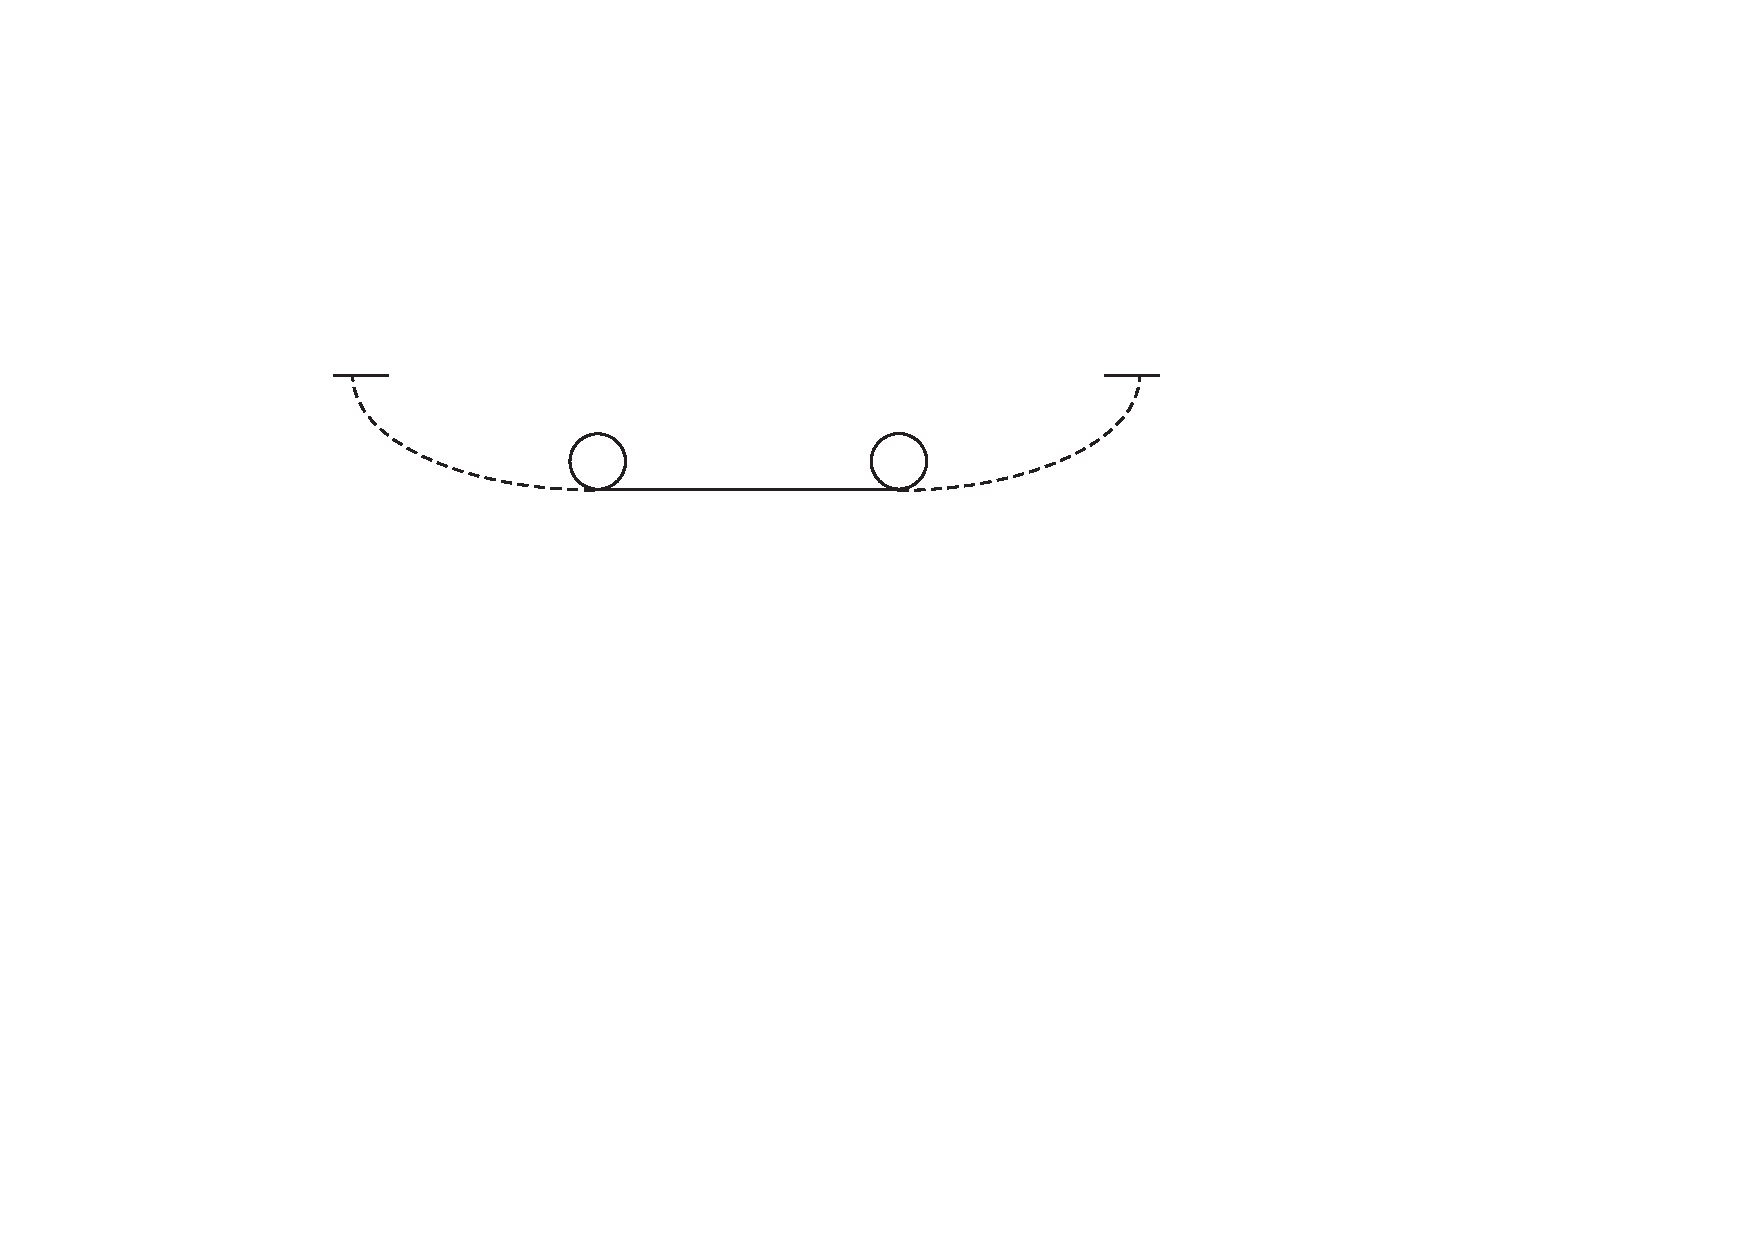
\includegraphics[width=0.6\textwidth]{%
gesamttex/edit_VIII,3/images/LH_37_05_153-154_d4_154r.pdf%
}} 
\vspace{0.5em}
\centerline{%
\lbrack\textit{Fig.~4}\rbrack%
}
% \newpage%
\vspace{1.5em}
%
\pstart
%
%
$A.e$, $B.f$.%
\pend
%
\pstart
\hspace{1mm}\hspace{-1mm}% Trick, weil \edlabel nicht zu \par-Beginn sein darf
\edlabel{37_05_153-154_11a}%
Celeritas corporis \textit{A}, est \textit{e}. 
Celeritas corporis \textit{B} est \textit{f}. 
Quod si celeritas corporis \textit{A} esset \textit{b} et corporis \textit{B} esset \textit{a}, 
%
forent vires\protect\index{Sachverzeichnis}{vis}
%
aequales seu potentiae\protect\index{Sachverzeichnis}{potentia} reciproce proportionales.%
\edlabel{37_05_153-154_11b}
%
\pend \pstart
%
Corpora vel sibi occurrunt, vel se sequuntur, si sibi occurrunt, 
%
\edtext{tunc vel sunt aequalia}{\lemma{tunc}\Bfootnote{\textit{(1)}~est majus m \textit{(2)}~vel~\textit{L}}} 
%
sunt aequalia vel inaequalia. 
Si sunt aequalia, tunc motu occurrunt vel aequali vel inaequali, si motu occurrant aequali habemus solutionem\lbrack,\rbrack\ si motu sibi occurrunt inaequali, tunc motus ipsius \textit{B} sit 
%
\edtext{celerior. Nempe}{\lemma{celerior.}\Bfootnote{\textit{(1)}~Ut autem \textit{(2)}~Nempe~\textit{L}}} 
%
erit ut $f+e$ ad \textit{e}. 
Quaeramus modum quo duo corpora quae 
%
\edtext{ambo sibi occurrant}{\lemma{ambo}\Bfootnote{\textit{(1)}~feruntur \textit{(2)}~sibi occurrant~\textit{L}}} 
%
celeritate \edtext{aequali, in navi,\protect\index{Sachverzeichnis}{navis}}{\lemma{}\Bfootnote{aequali, \textbar\ tamen \textit{gestr.}\ \textbar\ in navi,~\textit{L}}} 
%
accedente motu navis\protect\index{Sachverzeichnis}{motus navis} ferantur motu composito,\protect\index{Sachverzeichnis}{motus compositus} ita ut celeritas eorum sit ut $f+e$ ad \textit{e}. Sit celeritas 
%
\edtext{qua occurrere}{\lemma{qua}\Bfootnote{\textit{(1)}~concurrere \textit{(2)}~occurrere~\textit{L}}} 
%
finguntur \textit{g}, addatur illi motus navis \textit{n} et huic dematur, fiet $g+n$, et $g-n$. Et $g+n\,\sqcap\,f+e$ et $g-n\,\sqcap\,e$. 
\rule[0cm]{0mm}{18pt}Ergo $g\,\sqcap\,f+e-n$ ergo 
%
$\underset{\displaystyle g\phantom{x.x}}{\underbrace{f\,\ovalbox{\!$+e$}}-n}-n\,\sqcap\,\ovalbox{\textit{e}}$. 
%
Ergo $n\,\sqcap\,\displaystyle\frac{1}{2}f$. 
Ergo $g\,\sqcap\,e+\displaystyle\frac{1}{2}f$. 
Unde patet rem esse determinatam. Ut ergo rem tractemus generaliter sint 
\rule[0cm]{0mm}{10pt}corpora duo \textit{A}, \textit{B}, eorum celeritates ipsius \textit{B} 
%
\edtext{sit $+f$\lbrack,\rbrack\ ipsius \textit{A}}{\lemma{sit $+f$}\Bfootnote{\textit{(1)}~ipsius \textit{A} sit \textit{e} vel $-e$. Ponamus jam semper esse \textit{f} majus quam \textit{e}. Item alterum quod minorem habet motum, si non occurrit tunc motum ejus facia \textit{(2)}~ipsius \textit{A}~\textit{L}}} 
%
sit $-e$ si occurrit ipsi \textit{B}, sed $+e$, si ipsum antecedit, quia tamen minori celeritate praecurret, hinc semper faciamus \textit{e}, minorem quam \textit{f}, nam et si occurrunt sibi in nostra potestate est, 
%
\edlabel{37_05_153-154_5a}%
\edtext{}{% A-Footnote Randanmerkung
{\xxref%
{37_05_153-154_5a}{37_05_153-154_5b}}%
\lemma{}%
\Afootnote{%
\textit{Am unteren Blattrand}: %
(\protect\vphantom)Per has regulas id efficere possumus, ut datis duobus corporibus unoque facto %
(\protect\vphantom)dum scilicet feruntur reciproca moli %
celeritate\protect\index{Sachverzeichnis}{celeritates reciprocae moli}\lbrack\protect\vphantom()\rbrack,\textsuperscript{\lbrack a\rbrack} %
praedicamus alia, nam addemus tantum aut adimemus viam centri.\protect\index{Sachverzeichnis}{via centri}\lbrack\protect\vphantom()\rbrack
\newline\newline%Marginalienapparat:
{\footnotesize \textsuperscript{\lbrack a\rbrack} celeritate, \textit{(1)}~reliqua facilius \textit{(2)}~praedicamus~\textit{L}}}}%
quodnam eligere velimus pro affirmante vel 
%
\edlabel{37_05_153-154_4a}%
\edtext{}{% Neuer Absatz und Varianten
{\xxref%
{37_05_153-154_4a}{37_05_153-154_4b}}%
\lemma{negante.}%
\Bfootnote{%
\textbar\ Sit \textit{streicht Hrsg.}\ \textbar\ %
Ergo \lbrack154~v\textsuperscript{o}\rbrack\
\textbar\ celeritas \textit{erg.}\ \textbar\ %
\textit{A} sit $\pleibdashv e$.
\textit{(1)}~Deberet esse \textit{(2)}~Celeritas \textit{A} deberet esse \textit{(3)}~Fingatur~\textit{L}}}%
negante.%
\edlabel{37_05_153-154_5b}
\pend
%
\pstart
Ergo \lbrack154~v\textsuperscript{o}\rbrack\ celeritas \textit{A} sit $\pleibdashv e$. Fingatur%
\edlabel{37_05_153-154_4b}
%
$-bl$.
%
\pend
\pstart
.~.~.~.~.~.~.~.~.~.~.~.~.~.~.~.~\textit{B} 
%
\edtext{sit $+f$. Fingatur}{\lemma{sit $+f$.}\Bfootnote{\textit{(1)}~Deberet esse \textit{(2)}~.~.~.~.~.~.~.~.~.~. \textit{(3)}~Fingatur~\textit{L}}}
%
$+al$.
%
%
\pend
%
\vspace{0.5em} % evtl. entfernen
\pstart
\noindent
\lbrack\textit{Nachfolgend kleingedruckter Text gestrichen:}\rbrack % Petit-Passage
\pend
\vspace{0.5em}
\footnotesize
%
\pstart 
\noindent
%
Debet esse 
$f(\pleibdashv)n\,\sqcap\,al$.
Et $\pleibdashv e (\pleibvdash)n\,\sqcap\,bl$. 
%
\pend
%
\pstart\noindent
Ergo $(\pleibdashv)n\,\sqcap\,al-f$.
Et $\pleibdashv e \underset{\displaystyle (\leibvdash) n}{\underbrace{-al+f}}\,\sqcap\,-bl$. 
Ergo $al\,\sqcap\,\displaystyle\frac{\leibdashv e +f}{a-b}$ 
vel $bl\,\sqcap\,\pleibvdash\, e +al-f$.
Ergo $bl\,\sqcap\,\displaystyle\frac{b}{a-b}\overline{\leibdashv e +f}$\lbrack,\rbrack\ 
%
%
\edlabel{37_05_153-154_2a}%
\edtext{}{% NEUER ABSATZ UND VARIANTEN
{\xxref%
{37_05_153-154_2a}{37_05_153-154_2b}}%
\lemma{$\displaystyle\frac{a}{a-b}\overline{\leibdashv e +f}$.}%
\Bfootnote{%
\textit{(1)}~Ergo $n\,\sqcap$ \textit{(2)}~Ergo $al-bl\, \sqcap$ \textit{(3)}~Ergo~\textit{L}}}%
$al\,\sqcap\,\displaystyle\frac{a}{a-b}\overline{\leibdashv e +f}$.
\pend
%
\pstart \noindent
\rule[0cm]{0mm}{20pt}Ergo%
\edlabel{37_05_153-154_2b}
%
$(\pleibdashv) n\,\sqcap\,%
\edtext{\displaystyle\frac{\leibdashv ae \,\protect\ovalbox{\!$+af-af$}+bf}{a-b}$. 
Hinc}{\lemma{$\displaystyle\frac{\leibdashv ae \,\protect\ovalbox{\!$+af-af$}+bf}{a-b}$}\Bfootnote{\textit{(1)}~eritque \textit{(2)}~. Hinc~\textit{L}}}
%
si sit $\pleibdashv e\,\sqcap\,+e$, seu si corpora tendant in easdem partes fiet 
$(\pleibdashv) n \,\sqcap\,\displaystyle\frac{+ae+bf}{a-b}$ 
(\protect\vphantom)quae est ut obiter dicam celeritas 
%
\edtext{centri potentiae\protect\vphantom().\protect\index{Sachverzeichnis}{celeritas centri potentiae}}{\lemma{centri}\Bfootnote{\textit{(1)}~gravitatis \textit{(2)}~potentiae\protect\vphantom().~\textit{L}}}
%
Quod si ergo corpus quod sequitur nempe corpus \textit{B}, minus est corpore quod antecedit, \textit{A}, 
tunc: signum $(\pleibdashv)$ erit affirmativum,\protect\index{Sachverzeichnis}{signum affirmativum} et navis\protect\index{Sachverzeichnis}{navis} in eandem tendere intelligenda est
partem cum 
%
\edtext{corpore utroque;}{%
\lemma{}%
\Bfootnote{%
corpore \textbar~\textit{B} \textit{gestr.}~\textbar\ %
utroque;~\textit{L}}}
%
celeritate potentiae\protect\index{Sachverzeichnis}{potentia} per differentiam corporum divisae.
%
Si vero corpus sequens sit majus antecedente, in contrariam partem movenda est 
%
\edtext{navis,\protect\index{Sachverzeichnis}{navis} etiam}{\lemma{navis,}\Bfootnote{\textit{(1)}~denique si \textit{(2)}~etiam~\textit{L}}} 
%
differentia celeritatum,\protect\index{Sachverzeichnis}{differentia celeritatum} unde patet si sit $a\,\sqcap\,b$ non esse 
cur navis\protect\index{Sachverzeichnis}{navis} in hanc potius quam illam partem moveatur, adeoque quieturam. 
%
Hoc tamen aliunde videtur esse falsum,
%
ob signorum usum periculosum.\protect\index{Sachverzeichnis}{usus periculosus signorum}
%
\edtext{%		% C-Fn Stelle
Interea jam demonstratum
\edtext{aliunde}{\lemma{}\Bfootnote{aliunde \textit{erg.}~\textit{L}}}
est manifesto, viam navis\protect\index{Sachverzeichnis}{via navis} esse
%
\edtext{viam centri potentiae.\protect\index{Sachverzeichnis}{via centri potentiae}}{\lemma{}\Afootnote{\textit{Über} {\footnotesize viam centri potentiae}, \textit{ebenfalls gestrichen}:
\footnotesize{Imo error, non est totius potentiae,\protect\index{Sachverzeichnis}{potentia tota} sed solum ictus.\protect\index{Sachverzeichnis}{potentia ictus}}%
}}
%
Nam posito 
corporum concursu\protect\index{Sachverzeichnis}{concursus} 
%
per reciprocam celeritatem\protect\index{Sachverzeichnis}{celeritas reciproca} erit centrum potentiae\protect\index{Sachverzeichnis}{centrum potentiae} immobile in navi,\protect\index{Sachverzeichnis}{navis} 
feretur ergo tantum motu navis.\protect\index{Sachverzeichnis}{motus navis}}{%
\lemma{Interea \lbrack...\rbrack\ navis}%
\Cfootnote{%
Siehe die Passage auf S.~\refpassage{37_05_153-154_6a}{37_05_153-154_6b}.}}
%
\pend
%
\pstart
Video meum calculi errorem, debebam motum illum simpliciter 
%
\edtext{addere, sic}{%
\lemma{addere,}%
\Bfootnote{%
\textit{(1)}~sit %
\textit{(2)}~sic %
\textit{L}%
}}
%
ergo dicendum est
%
\rule[0cm]{0mm}{10pt}{\normalsize\lbrack\textit{Text bricht ab.}\rbrack}
%
\pend
\normalsize % normale Schriftgröße
\vspace{0.5em} % evtl. entfernen
%
%
\newpage
\pstart
%
Sit motus navis\protect\index{Sachverzeichnis}{motus navis} $(\pleibdashv)n$. Is addendus utrique, fiet 
$f(\pleibdashv)n\,\sqcap\,al$ et $\pleibdashv e (\pleibdashv)n\,\sqcap\,-bl$.
%
\pend \pstart\noindent
Ergo fiet: $(\pleibdashv)n\,\sqcap\,al-f$, 
et $\pleibdashv \underset{\displaystyle\overbrace{al-f}}{e(\leibdashv)n}\,\sqcap\,-bl$. 
Ergo $al+bl\,\sqcap\,f\,\pleibvdash\,e$ sive $l\,\sqcap\,\displaystyle\frac{f\,\leibvdash\,e}{a+b}$. %
\pend
%
\pstart\noindent
Ergo $al\,\sqcap\,\displaystyle\frac{a}{a+b}\smallfrown\overline{f\,\leibvdash\, e}$ et $bl\,\sqcap\,\displaystyle\frac{b}{a+b}\smallfrown f \,\pleibvdash\, e$ et 
%
$(\pleibdashv)n\,\sqcap\,\displaystyle\frac{\ovalbox{\textit{af}}\,\leibvdash ae\,\ovalbox{$-af$}-bf}{a+b}$. 
%
Hinc si corpora tendant in easdem partes fiet 
\rule[0cm]{0mm}{16pt}$(\pleibdashv)n\,\sqcap\,\displaystyle\frac{-ae-bf}{a+b}$. 
Videamus jam an ita sit $f\,\pleibdashv\, n\,\sqcap\,al$. Fiet: 
%
$\displaystyle\frac{af\,\ovalbox{$+bf$}-ae\,\ovalbox{$-bf$}}{a+b}\,\sqcap\,\displaystyle\frac{af-ae}{a+b}$, 
%
quod verum esse 
%
\edtext{patet, est}{\lemma{patet,}\Bfootnote{\textit{(1)}~sed in eo difficultas est quod videtur \textit{(2)}~est~\textit{L}}} 
%
autem \textit{f} 
%
\edtext{necessario major}{\lemma{necessario}\Bfootnote{\textit{(1)}~celerior \textit{(2)}~major~\textit{L}}} 
%
quam \textit{e}, quando corpus \textit{B} 
%
\rule[0cm]{0mm}{12pt}\edtext{persequitur. Et}{\lemma{persequitur}\Bfootnote{\textit{(1)}~vicissim \textit{(2)}~$(\pleibdashv)$ \textit{(3)}~. Et~\textit{L}}} 
%
proinde generaliter ex 
$f(\pleibdashv)n\,\sqcap\,al$ fiet:
%
$\displaystyle\frac{af\,\ovalbox{$+bf$}\,\leibvdash ae \,\ovalbox{$-bf$}}{a+b}\,\sqcap\,al\,\sqcap\,\displaystyle\frac{af \,\leibvdash\, ae}{a+b}$ 
%
et $\pleibdashv e (\pleibdashv)n\,\sqcap\,-bl$ dabit: 
%
$\displaystyle\frac{\ovalbox{$\leibdashv ae$}\,\leibdashv be \,\ovalbox{$\leibvdash ae$} -bf}{a+b}\,\sqcap\,\displaystyle\frac{-bf\,\leibdashv\, be}{a+b}$. 
%
\pend
%
\pstart
\rule[0cm]{0mm}{12pt}Calculus ergo verus est. 
Ac proinde si corpus unum \edtext{\textit{B}}{%
\lemma{}%
\Bfootnote{%
\textit{B} %
\textit{erg.~L}%
}}
%
aliud
%
\edtext{\textit{A}}{%
\lemma{}%
\Bfootnote{%
\textit{A} %
\textit{erg.~L}%
}}
%
insequatur, celerius quam movetur \textit{A}, tunc ut fiant celeritates potentiis reciprocae,\protect\index{Sachverzeichnis}{celeritates reciprocae potentiis} necessario retroagenda est navis.\protect\index{Sachverzeichnis}{navis} 
%
\edtext{Nam necessario}{\lemma{Nam}\Bfootnote{\textit{(1)}~ponamus corpus persequens esse minus \textit{(2)}~necessario~\textit{L}}} 
%
efficiendum est, ut corpus antecedens\protect\index{Sachverzeichnis}{corpus antecedens}
%
\edtext{retroagi videatur}{\lemma{retroagi}\Bfootnote{\textit{(1)}~intelligatur in nav \textit{(2)}~videatur~\textit{L}}} 
%
existentibus in navi.\protect\index{Sachverzeichnis}{navis} 
%
Hinc etiam patet esse \textit{n} summam\protect\index{Sachverzeichnis}{summa potentiarum applicata magnitudini corporum} vel 
%
\edtext{differentiam potentiarum applicatam}{\lemma{differentiam}\Bfootnote{\textit{(1)}~celeritatum divisam per \textit{(2)}~potentiarum \textit{(a)}~divisa \textit{(b)}~applicatam~\textit{L}}} 
%
magnitudini corporum,\protect\index{Sachverzeichnis}{differentia potentiarum applicata magnitudini corporum} 
%
seu motum navis\protect\index{Sachverzeichnis}{motus navis} esse viam centri gravitatis.\protect\index{Sachverzeichnis}{via centri gravitatis}
%
Hinc centrum gravitatis\protect\index{Sachverzeichnis}{centrum gravitatis} eadem semper procedit via, quia intelligitur procedere cum navi.\protect\index{Sachverzeichnis}{navis}
%
Hinc praeclare omnes difficultates solvuntur, patet enim
%
ex motuum compositione\protect\index{Sachverzeichnis}{compositio motuum}
%
quis sit ictus\protect\index{Sachverzeichnis}{ictus}\lbrack,\rbrack\ seu corpora in tantum in se invicem agere intelligi, 
%
\edtext{in quantum ictui\protect\index{Sachverzeichnis}{ictus}}{\lemma{in quantum}\Bfootnote{\textit{(1)}~sunt \textit{(2)}~ictui~\textit{L}}} 
%
resistunt,
%
%
reliqua motui ambobus communi\protect\index{Sachverzeichnis}{motus communis} tribuenda non pertinere ad actionem eorum in se
%
%
\edlabel{37_05_153-154_9a}%
\edtext{}{% B-Footnote
{\xxref%
{37_05_153-154_9a}{37_05_153-154_9b}}%
\lemma{$+al$}\Bfootnote{\textit{(1)}~Sit motus navis \textit{n}. \textit{(2)}~Post concursum manet \textit{n}~\textit{L}}}%
%
invicem.\protect\index{Sachverzeichnis}{actio corporum in se invicem}%
\pend
%
\pstart
Post concursum\protect\index{Sachverzeichnis}{concursus} manet \textit{n}%
\edlabel{37_05_153-154_9b}
%%
et quod ipsi \textit{e} addebatur ipsi \textit{f} detrahitur, vel contra.
%
Id est motus ante concursum\protect\index{Sachverzeichnis}{concursus} $f\,\sqcap\,+al(\pleibvdash)n$\lbrack,\rbrack\ $e\,\sqcap\,-bl(\pleibvdash)n$. 
%
%
\pend
%
\newpage
\pstart
\hspace{1mm}\hspace{-1mm}% Trick, weil \edlabel nicht zu \par-Beginn sein darf
\edlabel{37_05_153-154_7a}%
\edtext{}{% A-Footnote
{\xxref%
{37_05_153-154_7a}{37_05_153-154_7b}}%
\lemma{}\Afootnote{%
\textit{Hilfsrechnung am linken Blattrand}:\newline
$\protect\underset{\displaystyle \protect\overbrace{\leibvdash n -f}}{-al} \protect\underset{\protect \begin{array}{c}\protect\overbrace{\displaystyle -al+f} \\ \displaystyle +bl \,\leibdashv\, e \protect \end{array}}{(\leibvdash) n}\,\sqcap\,m\,\sqcap\,+f-2al\,\sqcap\,\leibdashv e + bl - al$.\newline
%
$\protect\underset{\displaystyle\protect\overbrace{\leibvdash\, e\, (\leibvdash)\, n}}{+bl} (\pleibvdash) n \,\sqcap\,i\,\sqcap\,\pleibdashv e+2bl\,\sqcap\,+f+bl-al$.\newline
%
$m\,\sqcap\,+f-2al\,\sqcap\, \protect\ovalbox{\textit{af}} +bf - \protect\ovalbox{2}\,af \,\pleibvdash\, 2ae \smallsmile a+b$.\newline
%
$i\,\sqcap\,\pleibdashv e +2bl\,\sqcap\,\pleibdashv\, ae \,\protect\ovalbox{$\leibdashv be$}+2bf\,\pleibvdash\, \protect\ovalbox{2}\,be\,\smallsmile\,a+b$.
}}%
Post concursum\protect\index{Sachverzeichnis}{concursus} fiet:%
\pend
%
\pstart\noindent 
%
\edtext{$\underset{\ \displaystyle i\,\sqcap\,(\leibvdash)2n \leibvdash e}{m\,\sqcap\,(\leibvdash)2n-f}$\lbrack,\rbrack}{%
\lemma{}%
\Bfootnote{%
$\protect\underset{\ \displaystyle i\,\sqcap\,(\leibvdash)2n \leibvdash e}{m\,\sqcap\,(\leibvdash)2n-f}$\lbrack,\rbrack\ %
\textit{erg.~L}%
}}
%
$\edtext{
\underset{\displaystyle\lbrack i\,\sqcap\rbrack\, +bl(\leibvdash)n}{m\,\sqcap\,-al(\leibvdash)n}$\lbrack,\rbrack
}{%
\lemma{}%
\Bfootnote{%
$i\,\sqcap$ \textit{erg.}\ \textit{Hrsg.}}}
%
seu $m\,\sqcap\,\displaystyle\frac{+bf-af\,\leibvdash\, 2ae}{a+b}$\lbrack,\rbrack\ $i\,\sqcap\,\displaystyle\frac{\leibdashv\, ae \,\leibvdash\, be +2bf}{a+b}$.%
\edlabel{37_05_153-154_7b}
%
%%
\pend
\count\Afootins=1200%
\count\Bfootins=1200%
\count\Cfootins=1200